\documentclass{beamer}

\usetheme{Copenhagen}

\title{The Euler Spiral}
\author{Max Mussavian}
\date[2022]{9th May 2022}
\begin{document}
\begin{frame}[plain]
    \maketitle
\end{frame}
\begin{frame}{Outline}
	\begin{itemize}
		\item Definitions and Derivations: Parametric Curves, Lengths and Curvature
		\item Relating the Curve Length to its Curvature
		\item Calculating Fresnel Integrals and the Euler Spiral
		\item Plotting the Euler Spiral and other Fun Curves
		\item Application: Designing Railways and Roads
	\end{itemize}
\end{frame}


\begin{frame}{Parametric Curves}
	
		All curves in this talk are in $\mathbb{R}^2$.
		\begin{definition}[A Parametric Curve]
			A parametric curve is a \alert{{smooth}} function that has the form
			$x = g(t)$ and $y=h(t)$ defined on an open interval $(a, b)$.
		
			The set of points traced out by the curve is called the trace.
		\end{definition}
	
\end{frame}

	\begin{frame}{How Long is a Curve?}
		\begin{figure}
		\centering
		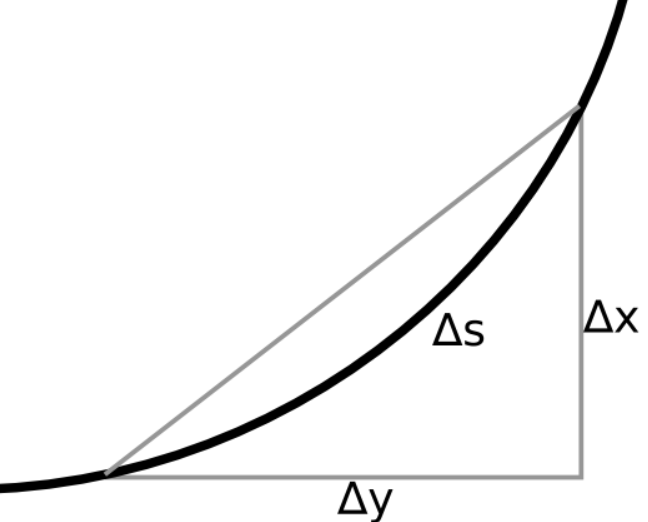
\includegraphics[width=50mm, scale=0.4]{arc_length_integral.png}
		\end{figure}
		\begin{itemize}
		\item Use Pythagoras to approximate $\Delta$s
		\item $\Delta s $ 
		$ \approx	\sqrt{\Delta y^2 + \Delta x^2} $
		\end{itemize}
	\end{frame}

\begin{frame}{Derivation Arc Length Integral}
	
	\begin{itemize}
		\item Write the whole Curve Length ,S, as a Riemann Sum and make it into Integral
		\item S $\approx$ $\sum\limits^{n}_{i=1}{\sqrt{\Delta y_i^2 + \Delta x_i^2}}$
		\item Factor out $\Delta x_i^2$
		\item S = ${\alert{\lim_{n \to \infty}}}\sum\limits^{n}_{i=1}{\sqrt{\Delta y_i^2/\Delta x_i^2 + 1}} \Delta x_i$
		\item S = $\int_{a}^{b} \sqrt{(dy/dx)^2+1}dx$
	\end{itemize}
\end{frame}

\begin{frame}{Derivation of Arc Length Integral}
	
	\begin{itemize}
		\item S = $\int_{a}^{b} \sqrt{(dy/dx)^2+1}dx$ 
		\item $\frac{dx/dt}{dx/dt}=1$ so
		\item S = $\int_{a}^{b} \sqrt{(\frac{dy/dt}{dx/dt})^2+(\frac{dx/dt}{dx/dt})^2}dx$
		\item Factor out $(\frac{dx/dt}{dx/dt})^2$ giving us:
		\item S = $\int_{a}^{b} \sqrt{(dy/dt)^2+(dx/dt)^2}dt$
	\end{itemize}
\end{frame}

\begin{frame}{Arc Length Integral}
	\begin{theorem}[Arc Length]
		The arc length between two points the curve for T = a and T = b is given by
		S = $\int_{a}^{b} \sqrt{(dy/dt)^2+(dx/dt)^2}dt$
	\end{theorem}
	\begin{figure}
		\centering
		\includegraphics[width=50mm, scale=0.4]{Arc length Integral.png}
	\end{figure}
\end{frame}

\begin{frame}{Deriving Formula for Curvature}
	\begin{columns}
		\begin{column}{0.4\textwidth}
			\begin{figure}
				\centering
				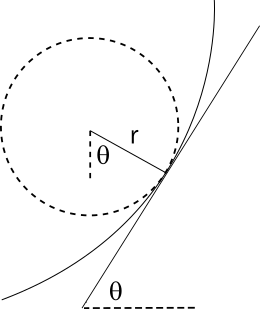
\includegraphics[width=50mm, scale=0.4]{illustration.png}
			\end{figure}
		\end{column}
		\begin{column}{0.6\textwidth}
			\begin{itemize}
				\item Firstly Curvature is 1/radius of Osculating Circle.
				\item Or the rate of Change of the angle the tangent makes with the x axis with respect to arc length.
				\item $ds=rd\theta$ $\implies$ $1/r=d\theta/ds$
				
				\item $\frac{ds}{dt} = \sqrt{x'^2+y'^2}$ from arc length.
				
				
			
			\end{itemize}
			
			
			
		\end{column}
	\end{columns}

	
\end{frame}

\begin{frame}{Deriving Formula for Curvature}
	\begin{itemize}
			\item $\tan \theta = \frac{y'(t)}{x'(t)}$ $\implies$ $\sec ^2 \theta \frac{d\theta}{dt} = \frac{x' y'' - y' x''}{x'^2}$.
			\item $sec^2\theta = tan^2\theta +1 = \frac{x'^2+y'^2}{x'^2}$ $\implies$
		$\frac{d\theta}{dt}=\frac{x' y'' - y' x''}{x'^2+y'^2}$
		
		
		
		\item Combining gives us
		$1/r= \frac{d\theta/dt}{ds/dt} = d\theta/ds = \frac{x' y'' - y' x''}{(x'^2+y'^2)^{3/2}}$
		
		\item Curvature, $\kappa$ = $\frac{x' y'' - y' x''}{(x'^2+y'^2)^{3/2}}$
	\end{itemize}
\end{frame}

\begin{frame}{How Curved is a Curve?}
	\begin{Theorem}[Curvature]
		The curvature of curve is $\kappa$ which is the reciprocal of the radius of the {\alert{osculating circle}} given by
		$\kappa=\frac{x' y'' - y' x''}{(x'^2+y'^2)^{3/2}}$
	\end{Theorem}
	\begin{figure}
	\centering
	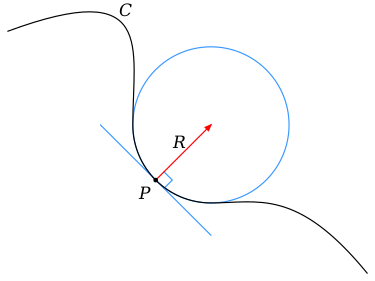
\includegraphics[width=50mm, scale=0.4]{Curvature_circle.png}
\end{figure}
\end{frame}

\begin{frame}{Circle}
	\begin{itemize}	
		
		\item Circle: The parametric equations for a circle with radius $r$ as $x(t)=r \cos(t)$ and $y(t)= r \sin(t)$. The arc length is 
		
		\[	
		s = \int_{0}^{2 \pi} \sqrt{r^2 \sin^2 t + r^2 \cos^2 t}dt = \left[r \right]_{0}^{2 \pi} = 2 \pi r
		\]
	
		\item Using the same Parametrisations we can work out the Curvature
		
		\[
		\kappa = \frac{r^2 \sin^2 t + r^2 \cos^2 t}{\left(r^2 \sin^2 t + r^2 \cos^2 t \right) ^ \frac{3}{2}} = \frac{1}{r}
		\]
		
	\end{itemize}
\end{frame}

\begin{frame}{Parabola Curve Length}
	\begin{itemize}	
			
			\item Parabola: We can define a parabola as $x(t)=t$ and $y(t)=t^2$. The arc length between 0 and 1 is 
			\begin{eqnarray*}
				s &=& \int_{0}^{1} \sqrt{1+4t^2}dt \\ &=& \left[\frac{1}{2} t\sqrt{1+ 4 t^2} +\frac{1}{4} \ln \left(2 t+\sqrt{1+ 4 t^2} \right) \right]_{0}^1 \\
				&\approx&	 1.48
			\end{eqnarray*}
		
	\begin{figure}
		\centering
		\includegraphics[width=50mm, scale=0.4]{Parabola_Arc_Length.png}
	\end{figure}
	\end{itemize}
\end{frame}

\begin{frame}{Parabola Curvature}
	\begin{itemize}	
		
		\item Parabola: Recall $x(t)=t$ and $y(t)=t^2$. 
		
		\[
		\kappa = \frac{2}{\left(1 + 4t^2 \right) ^ \frac{3}{2}}
		\]
		
	\begin{figure}
	\centering
	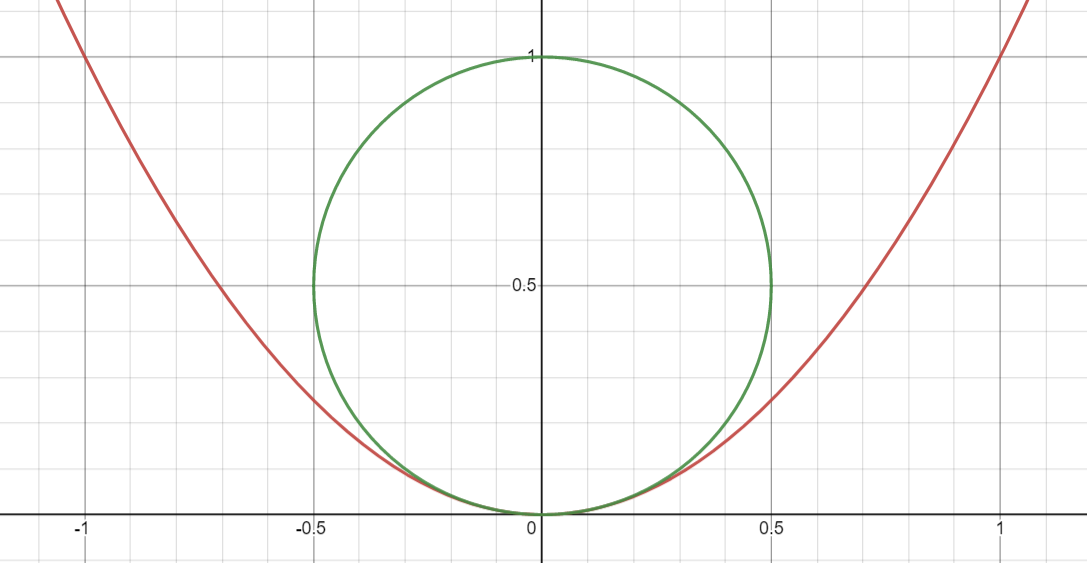
\includegraphics[width=50mm, scale=0.4]{Parabola.png}
\end{figure}

	\end{itemize}
\end{frame}

\begin{frame}{Relating Curve Length to Curvature}
	Let's try the following parametrisation for $x$ and $y$
	\begin{eqnarray*}
		x(t) &=& \int_{0}^{t} \cos f(u) du \\
		y(t) &=& \int_{0}^{t} \sin f(u) du
	\end{eqnarray*}
	This gives us
	\begin{eqnarray*}
		x' = x'(t) = \cos f(t) &\mbox{ and }& x''=-f'(t) \sin f(t) \\
		y' = y'(t) = \sin f(t) &\mbox{ and }& y''=f'(t) \cos f(t)
	\end{eqnarray*}
\end{frame}

\begin{frame}{Relating Curve Length to Curvature}
	This gives us the following for slope, arc length and curvature
	\begin{eqnarray*}
	\frac{dy}{dx} &=& \frac{\sin f(t)}{\cos f(t)} = \tan f(t) \\
 	s &=& \int_0^t \sqrt{\cos^2 f(u) + \sin^2 f(u)} du = t \\
 	\kappa &=& \frac{f'(t) \cos^2 f(t) + f'(t) \sin^2 f(t)}{\cos^2 f(t) + \sin^2 f(t)} = f'(t)
 \end{eqnarray*}
\end{frame}

\begin{frame}{Define the Curve by Curve Length and Curvature}
	We can replace the variable $t$ by the arc length $s$.
	 
	And the curvature at point $t$ is $f'(t)$. Which means
	 \[
	 f(t) = \int \kappa(t) dt
	 \]
	Thus the equations for the curve become
	\begin{eqnarray*}
	x = x(s) &=& \int_{0}^{s} \cos \left( \int_0^u \kappa(t) dt \right) du \\
	y = y(s) &=& \int_{0}^{s} \sin \left( \int_0^u \kappa(t) dt \right) du
	\end{eqnarray*}
	Hence the curve is defined by arc length and curvature alone.
\end{frame}

\begin{frame}{A Very Simple Example}
	We can make the curvature $\kappa$ constant and equal to 1. Then 
	$ \int_0^u \kappa(t) dt = u $ and
	\begin{eqnarray*}
		x = x(s) &=& \int_{0}^{s} \cos u du = \sin s\\
		y = y(s) &=& \int_{0}^{s} \sin u du = - \cos s + 1
	\end{eqnarray*}
	which is the parametric curve for a circle with centre $(0, 1)$ and radius $1$.
	
\end{frame}


\begin{frame}{The Euler Spiral}
	Recall: Euler defined his curve as one where the curvature is proportional to arc length.
	
	\begin{center}
		\boxed{\kappa(s) = s}
	\end{center}
	Then 
	$ \int_0^u \kappa(t) dt = \frac{u^2}{2} $ and
	\begin{eqnarray*}
		x = x(s) &=& \int_{0}^{s} \cos \frac{u^2}{2} du\\
		y = y(s) &=& \int_{0}^{s} \sin \frac{u^2}{2} du
	\end{eqnarray*}

	But since these integrals can't be solved analytically how were they calculated?
\end{frame}

\begin{frame}{Solving the Integrals: Euler}
	\begin{itemize}
		\item In 1744 Euler derived these integrals.
		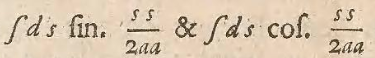
\includegraphics[width=50mm, scale=0.5]{euler_scripture_1.png}	
		\item He derived a series expansion which is still a viable method for small $s$.
		
		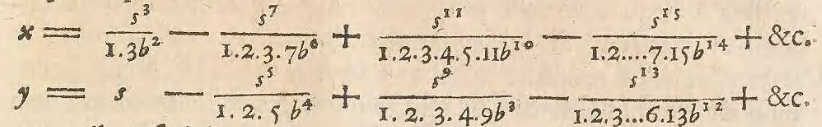
\includegraphics[width=100mm, scale=0.7]{euler_scripture.png}
		
		\item In 1781 he proved the integrals for limits between 0 and $\infty$ are equal to  $\frac{a \sqrt{\pi}}{2}$ 
	\end{itemize}
\end{frame}

\begin{frame}{Solving the Integrals: Fresnel and Cornu}
	\begin{itemize}
		\item In 1818 Augustin Fresnel rediscovered these integrals when he investigated the diffraction of light through a slit. He showed that the intensity (under some assumptions) was 
		\[
		\left( \int_{0}^{s}\cos \left( \pi t^2 / 2 \right) dt \right) ^2 + 
		\left( \int_{0}^{s}\sin \left( \pi t^2 / 2 \right) dt \right) ^2
		\] 
		\item Up to a factor of $\pi$ the integrals are the same as the ones Euler derived.
		\item These integrals are now called the \emph{Fresnel Integrals}.
		\item Fresnel calculated them for values of $s$ between 0.1 and 5.1.
	\end{itemize}
\end{frame}

\begin{frame}{Solving the Integrals: Today with Python}
	\begin{columns}
		\begin{column}{0.5\textwidth}
			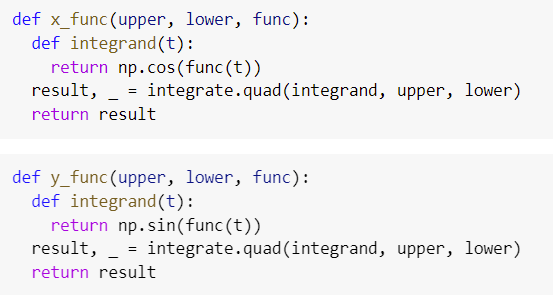
\includegraphics[width=50mm, scale=0.5]{code_1.png}
			
			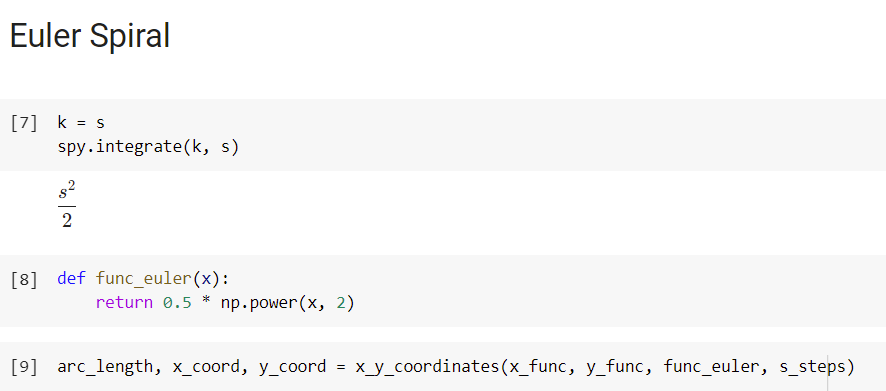
\includegraphics[width=50mm, scale=0.5]{code_2.png}
		\end{column}
		\begin{column}{0.5\textwidth}
		Nowadays we use computers and numerical methods to evaluate these integrals.
			
		\end{column}
	\end{columns}
\end{frame}

\begin{frame}{The Euler Spiral - $x$ $y$ Coordinates}
	\begin{figure}
		\caption{Fresnel Integrals with arguments $\frac{u^2}{2}$}
		\centering
		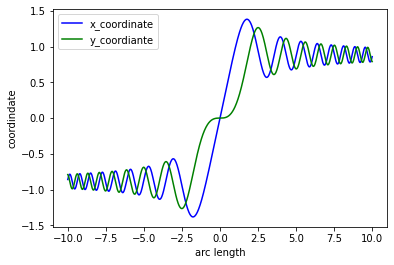
\includegraphics[width=70mm, scale=0.5]{euler_x_vs_y.png}
	\end{figure}
	As expected these converge to $\pm \frac{\sqrt{\pi}}{2} \approx 0.8862$.
\end{frame}

\begin{frame}{The Euler Spiral}
	\begin{figure}
		\caption{The Euler Spiral aka Cornu Curve}
		\centering
		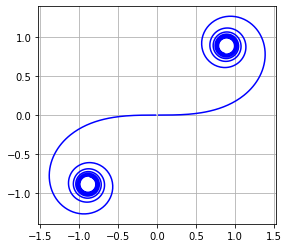
\includegraphics[width=70mm, scale=0.5]{euler_spiral.png}
	\end{figure}
	
\end{frame}

\begin{frame}{Eulers First Drawing}
\begin{figure}
	\centering
	\begin{minipage}{.5\textwidth}
		\centering
		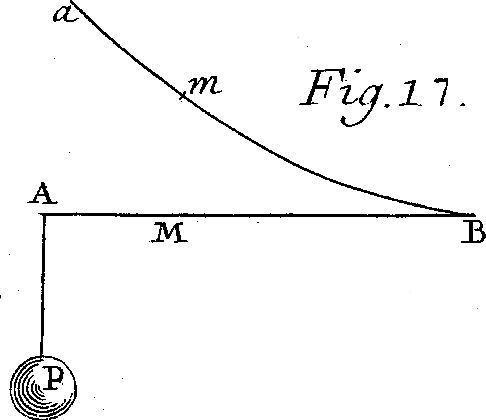
\includegraphics[width=.8\linewidth]{Euler_first_drawing.png}
		\caption{Euler's First Drawing from a 1744 Publication. P refers to a weight.}
		\label{fig:test1}
	\end{minipage}%
	\begin{minipage}{.5\textwidth}
		\centering
		\includegraphics[width=0.9\linewidth]{Euler second drawing.png}
		\caption{Euler's drawing of full Spiral in 1781 after solving integrals to $\infty$}
		\label{fig:test2}
	\end{minipage}
\end{figure}
\end{frame}

\begin{frame}{Other Fun Curves: Even Powers of $s$}
	\begin{figure}
		\caption{$\kappa(s) = s^2$}
		\centering
		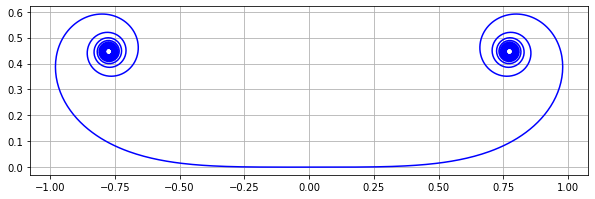
\includegraphics[width=85mm, scale=0.5]{chaise_longue.png}
	\end{figure}
\end{frame}

\begin{frame}{More Fun Curves: Mix in a Bit of a Circle}
	\begin{figure}
		\caption{$\kappa(s) = s ^ 2 -2.19$}
		\centering
		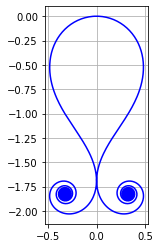
\includegraphics[width=35mm, scale=0.2]{s_squared_minus_219.png}
	\end{figure}
\end{frame}

\begin{frame}{More Fun Curves: Polynomials}
	\begin{figure}
		\caption{$\kappa(s) = 5 s ^ 4 - 18 s ^ 2 + 5$}
		\centering
		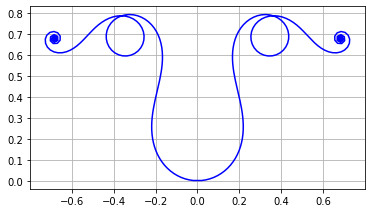
\includegraphics[width=70mm, scale=0.5]{five_s^4.png}
	\end{figure}
\end{frame}

\begin{frame}{More Fun Curves: Trigonometric Functions}
	\begin{figure}
		\caption{$\kappa(s) = \cos(s) - s \sin(s)$}
		\centering
		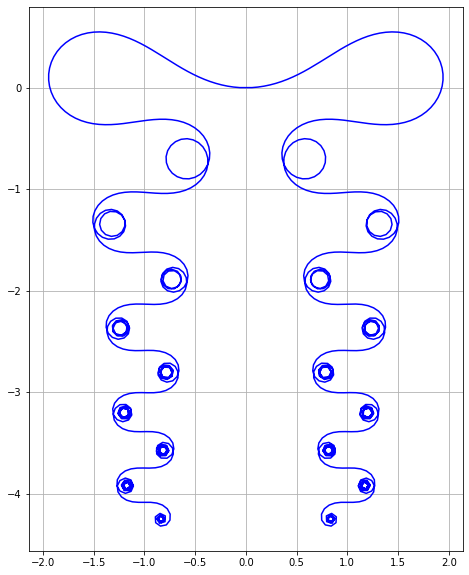
\includegraphics[width=50mm, scale=0.2]{elegant_madness.png}
	\end{figure}
\end{frame}
	
\begin{frame}{More Fun Curves: Hyperbolic Functions}
	\begin{figure}
		\caption{$\kappa(s) = \sinh(s) - 5.19$}
		\centering
		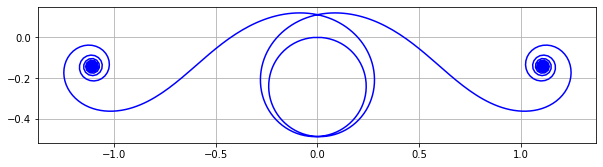
\includegraphics[width=100mm, scale=0.5]{sinh.png}
	\end{figure}
\end{frame}

\begin{frame}{A major use of the Euler Spiral}
	\begin{itemize}
		\item As trains became faster in the 19th century, the Euler spiral was rediscovered by railway designers.
		\item Railway engineers discovered that a track shape with gradually varying curvature provided a smooth riding experience.
		\item In 1899 railway engineer Arthur Talbot solved the problem mathematically and derived the same integrals as Fresnel.
		\item His solution was ``a curve whose degree-of-curve increases directly along the curve."
		\item He derived a series expansion for the integrals almost identical to Euler's 1744 series. 
	\end{itemize}
\end{frame}

\begin{frame}{Designing Roads and Railways}
	\begin{itemize}
		\item Transition curves are used to link straight sections of motorways or railways.
		\item They are designed to give passengers a smooth ride with no sudden changes in acceleration.

	\end{itemize}
		\begin{figure}
		\caption{Cloverleaf Motorway Interchange}
		\centering
		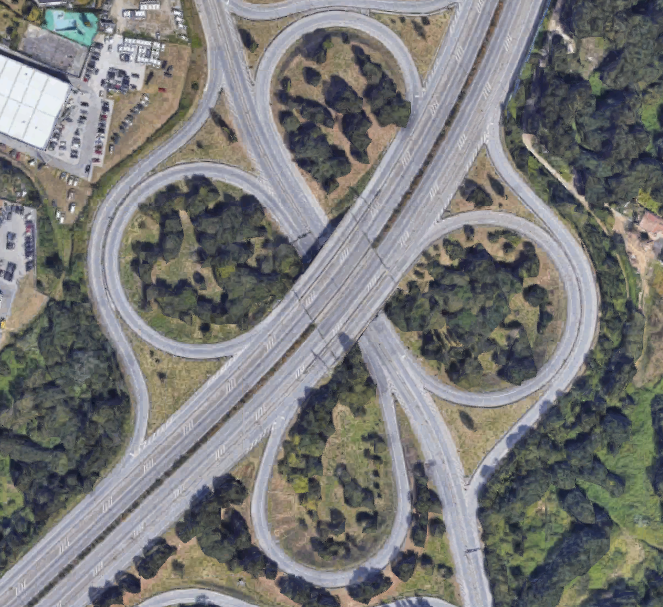
\includegraphics[width=50mm, scale=0.5]{cloverleaf_motorway.png}
	\end{figure}

\end{frame}

\begin{frame}{Why Transition Curves are Euler Spirals}
	\begin{itemize}
	\item The acceleration along the transition curve is given by
 	 \[
 	 a=s''(t) \vec{T}+\kappa s'(t)^2 \vec{N}
 	 \]
 	 Where $\vec{T}$ is the unit tangent vector and $\vec{N}$ is the unit normal vector.
 	 \item If the car/train is going round the curve at constant speed $s'(t)=constant$ and $s''(t)=0$.	
 	 \item The acceleration at constant speed only depends on the curvature $\kappa$ and speed $s'(t)$ in the direction of the normal vector.
	\end{itemize}
\end{frame}

\begin{frame}{Case 1: Semicircular Transition Curves}
	A closed  track is made up of four segments.
	\begin{enumerate}
		\item A straight track of length 1km
		\item A semicircular track of length 1km. This has radius $1,000 / \pi m \approx 318.31m$
		\item A straight track of length 1km
		\item A semicircular track of length 1km.
	\end{enumerate}
	Let the vehicle go around the track at a constant speed of $60 km/h = 16 \frac{2}{3} m/s$.
\end{frame}

\begin{frame}{Case 1: Position and Acceleration}
	\begin{columns}
		\begin{column}{0.8\textwidth}			
			\begin{figure}
				\caption{Position and Acceleration}
				\centering
				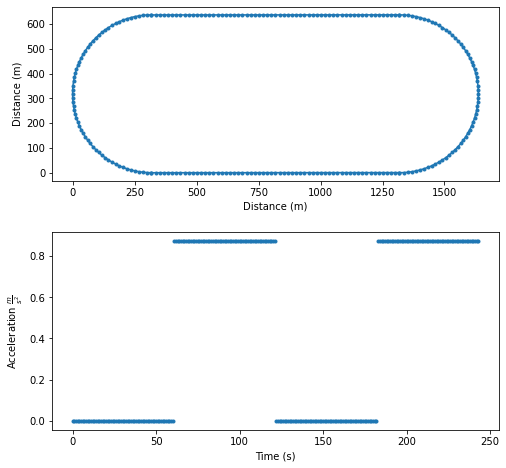
\includegraphics[width=70mm, scale=0.2]{circular_track.png}
			\end{figure}
		\end{column}
		\begin{column}{0.33\textwidth}
			Note: The acceleration is a step function. 
			
			
			As a passenger you would feed the full centrifugal force ({\alert{$F=mv^2/r$}}) pushing you outward the moment you entered the curve. 		
		\end{column}
	\end{columns}
\end{frame}


\begin{frame}{Case 2: Euler Spiral Transition Curves}
	\begin{itemize}
		\item A closed track with same width and height. 
		\item Replace semicircles with two parts of an Euler Spiral.
		\item Recall that the curvature is proportional to arc length. $\kappa = \alpha s $ for some $\alpha$.
		\item The width and height of an Euler Spiral that turns through $\pi/2$ is given by 
		\begin{eqnarray*}
			width &=& \sqrt{\pi / \alpha} C(1) \\
			height &=& \sqrt{\pi /\alpha}S(1)
		\end{eqnarray*}
		where $S(u)$ and $C(u)$ are the standard Fresnel integrals.
	
	\end{itemize}
	
	\[
	\alpha = \frac{\pi S(1)^2}{r^2} \approx 5.95 \times 10 ^{-6}
	\]
	
\end{frame}

\begin{frame}{Case 2: Euler Spiral Transition Curves}
	\begin{columns}
		\begin{column}{0.8\textwidth}			
			\begin{figure}
				\caption{Position and Acceleration}
				\centering
				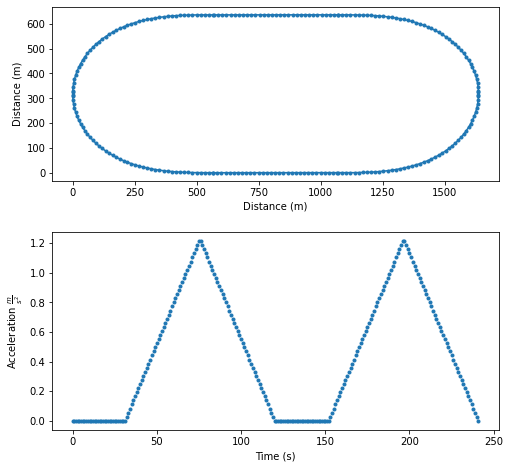
\includegraphics[width=70mm, scale=0.2]{euler_track.png}
			\end{figure}
		\end{column}
		\begin{column}{0.33\textwidth}
			Note: The acceleration increases linearly as we move through the curve.
			
			The maximum acceleration however at the apex is greater than with the semicircular track. But the ride is more comfortable now!
					
		\end{column}
	\end{columns}

\end{frame}



\begin{frame}
	\centering
	Thanks for listening!
	 
\end{frame}

\end{document}
